\section{Physikalischer Hintergrund}
\subsection{Dosisgrößen}
Wir definieren nun die wesentlichen Größen zur Charakterisierung der Wechselwirkung/Schädigung von Materie mit ionisierender Strahlung:\\
Die \underline{Dosis D} ist ein Maß des Energieübertrags $\mathrm{d}E$ ionisierender Strahlung auf ein Materie-Massenelement $\mathrm{d}m$:
\begin{equation}\label{eq:dosis}
	D = \frac{\mathrm{d}E}{\mathrm{d}m},\ [D] = J/kg \equiv Gy\ \textrm{(Gray)}
\end{equation}
Die zeitliche Änderung der Dosis $\dot{D}$ nennt man \underline{Dosisleistung}.\\
Will man berücksichtigen, dass die Schädigung biologischen Gewebes sowohl von der Strahlungsart R als auch von der Gewebeart T abhängt, führt man die Wichtungsfaktoren $w_R$ und $w_T$ ein, um die für den Strahlenschutz wesentliche Messgröße der \underline{effektiven (Äquivalent-)Dosis $H_E$} zu definieren:
\begin{equation}
	H_E = \sum_{R,T} w_R \cdot w_T \cdot D_{R,T},\ [H_E]=J/kg \equiv Sv\ \textrm{(Sievert)}
\end{equation}
Dabei findet man, dass die Dosisleistung einer Punktquelle mit dem Quadrat des Abstandes zu dieser fällt:
\begin{equation*}
		\dot{D} \propto \frac{1}{d^2}
\end{equation*}
Diesen Zusammenhang nennt man \textbf{Abstandsquadratgesetz}.\cite{PA_neu}

\subsection{Aktivität}
Um die Dosisleistung für die gegebenen $\gamma$-Strahler in Aufgabe 2.3 abzuschätzen, benötigen wir die \underline{Aktivität A} als Maß für die Anzahl der spontanen Kernumwandlungen pro Zeiteinheit. Mit dem exponentiellen Zerfallsgesetz erhalten wir:
\begin{equation} \label{eq:aktivitaet}
	A(t)=A(t=0) \cdot \left(\frac{1}{2}\right)^{\frac{t}{T_{1/2}}}, [A] = 1/s \equiv Bq \textrm{(Bequerel)}
\end{equation}
Hier bei ist $T_{1/2}$ die Halbwertszeit des gegebenen Isotops.\cite{PA_RM1}

\subsection{Messprinzip: Ionisationskammer}
Grob gesprochen ist eine Ionisationskammer ein (beliebig geformter) Kondensator, dessen Dielektrikum gasförmig (in unserem Fall Luft) vorliegt. Tritt ionisierende Strahlung (Primärteilchen) in das Kammervolumen, so entstehen durch Wechselwirkung - in unserem Falle durch inkohärente Streuung und Photoeffekt - mit den Gasteilchen Elektronen-Ionen-Paare (Sekundärteilchen), indem die Elektronen aus der Atomhülle des bindenden Atoms herausgeschlagen werden. Diese Ladungsträger gelangen nun im Idealfall durch Coulomb-Wechselwirkung zu einer Kondensatorplatte, wo sie nun als Stromfluss I nachgewiesen werden können. Für näherungsweise konstante Dosisleistungen im Zeitintervall $\Delta t$ erhalten wir die Proportionalität zwischen dem Stromfluss und der Dosis:

\begin{equation} \label{eq:Ionenkammer}
	D(t) = D(t_0) + \int \limits_{t_0}^{t} \dot{D}(\tau) \mathrm{d}\tau \propto I
\end{equation}
\ \\
Ist die Kondensatorspannung (und somit auch die Feldstärke) zu niedrig, bewegen sich die geladenen Teilchen zu langsam und die Rekombinations-Wahrscheinlichkeit steigt. Ist sie andererseits zu groß, werden die Primärteilchen zu stark beschleunigt, sodass sie lawinenartig weitere Ionisationen auslösen und Sekundärladungsträger erzeugen. Beide Fälle würden die Messung verfälschen, wodurch man eine Kompromisslösung im sogenannten Sättigungsbereich finden muss.

\ \\
In Gleichung \ref{eq:Ionenkammer} sehen wir die Abhängigkeit der Dosis von der Dichte des Dielektrikums $\rho$. Da die Dichte der Luft in unserem Detektor vom Druck p, der Temperatur T und der Luftfeuchte f abhängt, müssen wir diese Einflüsse eventuell korrigieren:
\begin{equation}
	\rho = \rho_0 \cdot \frac{T_0}{T} \cdot \frac{p}{p_0} ,
	\ T_0 = 293,15\ K,\ p_0 = 101,3\ kPa, \rho_0 =1,20 \frac{kg}{m^3}
    \label{formel:kappa}
\end{equation}
Wobei $\rho_0$ der Dichte von Luft bei Normbedingungen entspricht. Den Einfluss der Luftfeuchte wollen wir an dieser Stelle vernachlässigen. \cite{PA_neu}


\subsection{Optisch stimulierte Lumineszenz}

Die Funktionsweise der optisch stimulierten Lumineszenz kann über ein Bändermodell erklärt werden. Grundsätzlich beschreibt das Phänomen der Lumineszenz die Lichtemission beim Übergang eines physikalischen Systems von einem angeregten in seinen Grundzustand.
Die Anregung des Systems kann beispielsweise durch Strahlung erfolgen. Typischerweise tritt dieses Phänomen bei elektrischen Isolatoren auf.\\
Unregelmäßigkeiten im Kristallgitter erzeugen zwischen Leitungs- (LB) und Valenzband (VB) zusätzliche Energieniveaus. Unterhalb der Fermi-Energie heißen diese Niveaus Aktivatorterme, oberhalb davon Haftterme. 

\begin{center}
    \minipanf    
    \makebox[\textwidth]{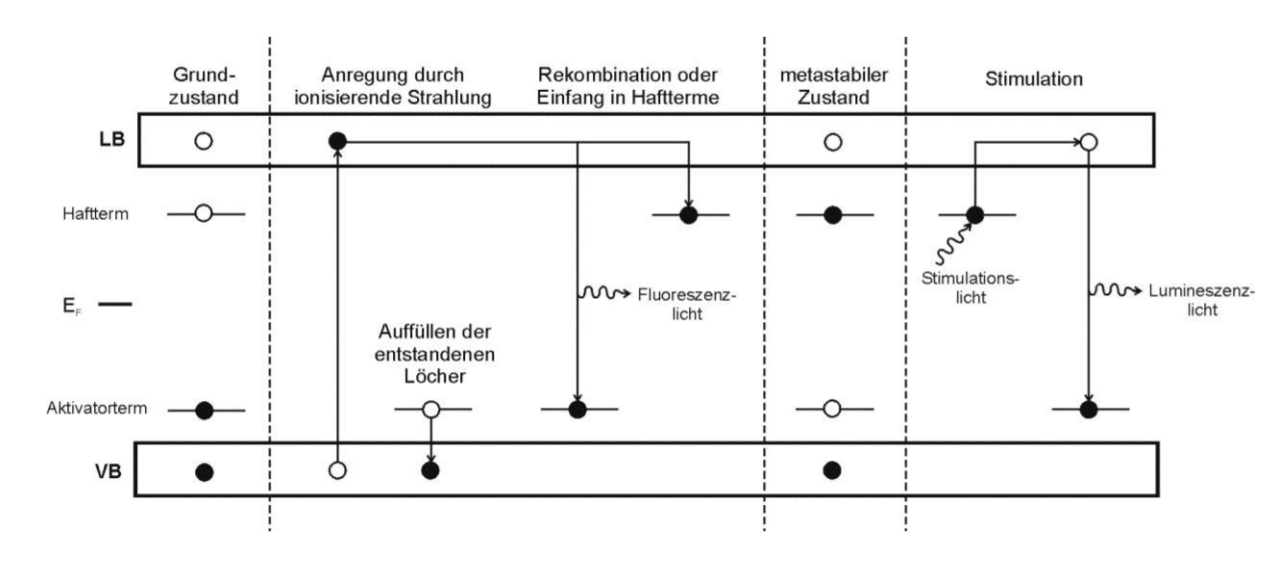
\includegraphics[width=1.1\linewidth, height=0.35\textheight]{pic/baendermodell}}
    \captionof{figure}{Schema zur optisch stimulierten Lumineszenz \cite{PA_neu}}
    \label{fig:band}
    \minipend
\end{center}

Im Grundzustand befinden sich Elektronen nur im Valenzband und den Aktivatortermen.
Regt man das System allerdings an, zum Beisiel durch ionisierende Strahlung, können einige Elektronen vom Grundzustand auf das Leitungsband oder die Hafterme springen. Aus dem Leitungsband springen sie entweder direkt un den Grundzustand, wobei sie Licht emittieren, oder fallen zunächst auf den metastabilen Zustand im Haftterm, der die Elektronen einige Zeit speichert.
Fällt nun Licht mit einer speziellen Wellenlänge auf das zuvor bestrahlte Material, springen die Elektronen aus den Hafttermen in das Leitungsband und fallen von dort meist in den Grundzustand, wobei sie Licht emittieren. \cite{PA_alt}

\subsection{BeO$max$-Funktionsprinzip}
Wir benutzen hier passive Sonden aus Berylliumoxid als Leuchtstoff. Diese Verbindung hat eine effektive Ordnungszahl von 7,13, was eine hohe Ähnlichkeit zu menschlichem Gewebe (Weichteile: 7,42, Knochen: 10) darstellt und deshalb ähnliche Absorptionseigenschaften besitzt.
Man bestrahlt die Sonden für ein zuvor berechnetes Zeitintervall. Danach sollte eine Abklingzeit von ca. 15 Minuten eingehalten werden, ehe die Sonden belichtet und ausgelesen werden. Damit wird ein Rauschen vermieden und sichergestellt, dass nur die in den Hafttermen gespeicherten Elektronen eine Rolle bei der Erzeugung des Lumineszenzlichtes spielen, bevor die Haftterme optisch angeregt werden.\\
Die passiven Sensoren haben jeder für sich ein spezifisches Ansprechvermögen, welches aus einem Signal vor der Bestrahlung, sowie nach der Bestrahlung und einer bekannten Referenzdosis bestimmt werden kann. Das Signal aus der Nullmessung ändert sich nach jeder optischen Stimulation und muss von Chip zu Chip und Messung zu Messung immer neu bestimmt werden. Damit berechnet sich das Ansprechvermögen folgendermaßen:

\begin{equation} \label{eq:ansprechvermoegen}
    \epsilon = \frac{LS_R - LS_{R,0}}{D_R}
\end{equation}
\ \\
Dabei beschreiben LS$_R$ das Lichtsignal aus der Messung bekannter Dosis, LS$_{R,0}$ das Nullsignal und D$_R$ die Referenzdosis.
Nachfolgende Gleichung beschreibt die Errechnung der Dosis aus den Lichtsignalen der Nullmessung, der Messung nach der Bestrahlung und dem Ansprechvermögen: \cite{PA_alt}
\begin{equation}
    D = \frac{LS - LS_0}{\epsilon}
\end{equation}